\documentclass{standalone}
\usepackage{tikz}

\begin{document}
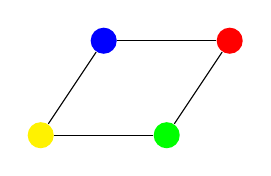
\begin{tikzpicture}[scale=0.8]
    % Nodes
    \node (A) at (0,0) [circle, fill=blue] {};
    \node (B) at (2,0) [circle, fill=red] {};
    \node (C) at (1,-1.5) [circle, fill=green] {};
    \node (D) at (-1,-1.5) [circle, fill=yellow] {};

    % Edges
    \draw (A) -- (B);
    \draw (B) -- (C);
    \draw (C) -- (D);
    \draw (D) -- (A);

    % Adding an edge will increase the chromatic number
\end{tikzpicture}
\end{document}